\documentclass[11pt,a4paper]{article}
% ============================================================
% Shared preamble for Claude Experiments reports (Ukrainian, LuaLaTeX)
% Compile with: lualatex report_*_uk.tex
% Include this AFTER \documentclass in each report:
%   \documentclass[11pt,a4paper]{article}
%   % ============================================================
% Shared preamble for Claude Experiments reports (Ukrainian, LuaLaTeX)
% Compile with: lualatex report_*_uk.tex
% Include this AFTER \documentclass in each report:
%   \documentclass[11pt,a4paper]{article}
%   % ============================================================
% Shared preamble for Claude Experiments reports (Ukrainian, LuaLaTeX)
% Compile with: lualatex report_*_uk.tex
% Include this AFTER \documentclass in each report:
%   \documentclass[11pt,a4paper]{article}
%   \input{../preamble_uk}
% ============================================================
% Cyrillic via LuaLaTeX + fontspec (pdflatex has no T2A here).
\usepackage{fontspec}
\setmainfont{DejaVu Serif}
\setsansfont{DejaVu Sans}
\setmonofont{DejaVu Sans Mono}
\usepackage[a4paper,top=2.5cm,bottom=2.5cm,left=2.5cm,right=2.5cm]{geometry}
\usepackage{amsmath,amssymb}
\usepackage{graphicx}
\usepackage{subcaption}
\usepackage{booktabs}
\usepackage{xcolor}
\usepackage[colorlinks=true,allcolors=blue]{hyperref}
\usepackage{microtype}
\usepackage{float}
\usepackage{array}
\microtypesetup{expansion=false}

% Color scheme
\definecolor{colMicro}{HTML}{222222}
\definecolor{colExact}{HTML}{2878b5}
\definecolor{colPlacement}{HTML}{e07a1f}
\definecolor{colBoundary}{HTML}{429c74}
\definecolor{colCurrent}{HTML}{c23b55}
\definecolor{colMM}{HTML}{c23b55}

\providecommand{\SIG}{\textcolor{green!50!black}{\textbf{*}}}
\providecommand{\NS}{\textcolor{gray}{n.s.}}
\providecommand{\DRMS}{\Delta\mathrm{RMST}}
\providecommand{\ci}[2]{$[{#1},\;{#2}]$}

% ============================================================
% Cyrillic via LuaLaTeX + fontspec (pdflatex has no T2A here).
\usepackage{fontspec}
\setmainfont{DejaVu Serif}
\setsansfont{DejaVu Sans}
\setmonofont{DejaVu Sans Mono}
\usepackage[a4paper,top=2.5cm,bottom=2.5cm,left=2.5cm,right=2.5cm]{geometry}
\usepackage{amsmath,amssymb}
\usepackage{graphicx}
\usepackage{subcaption}
\usepackage{booktabs}
\usepackage{xcolor}
\usepackage[colorlinks=true,allcolors=blue]{hyperref}
\usepackage{microtype}
\usepackage{float}
\usepackage{array}
\microtypesetup{expansion=false}

% Color scheme
\definecolor{colMicro}{HTML}{222222}
\definecolor{colExact}{HTML}{2878b5}
\definecolor{colPlacement}{HTML}{e07a1f}
\definecolor{colBoundary}{HTML}{429c74}
\definecolor{colCurrent}{HTML}{c23b55}
\definecolor{colMM}{HTML}{c23b55}

\providecommand{\SIG}{\textcolor{green!50!black}{\textbf{*}}}
\providecommand{\NS}{\textcolor{gray}{n.s.}}
\providecommand{\DRMS}{\Delta\mathrm{RMST}}
\providecommand{\ci}[2]{$[{#1},\;{#2}]$}

% ============================================================
% Cyrillic via LuaLaTeX + fontspec (pdflatex has no T2A here).
\usepackage{fontspec}
\setmainfont{DejaVu Serif}
\setsansfont{DejaVu Sans}
\setmonofont{DejaVu Sans Mono}
\usepackage[a4paper,top=2.5cm,bottom=2.5cm,left=2.5cm,right=2.5cm]{geometry}
\usepackage{amsmath,amssymb}
\usepackage{graphicx}
\usepackage{subcaption}
\usepackage{booktabs}
\usepackage{xcolor}
\usepackage[colorlinks=true,allcolors=blue]{hyperref}
\usepackage{microtype}
\usepackage{float}
\usepackage{array}
\microtypesetup{expansion=false}

% Color scheme
\definecolor{colMicro}{HTML}{222222}
\definecolor{colExact}{HTML}{2878b5}
\definecolor{colPlacement}{HTML}{e07a1f}
\definecolor{colBoundary}{HTML}{429c74}
\definecolor{colCurrent}{HTML}{c23b55}
\definecolor{colMM}{HTML}{c23b55}

\providecommand{\SIG}{\textcolor{green!50!black}{\textbf{*}}}
\providecommand{\NS}{\textcolor{gray}{n.s.}}
\providecommand{\DRMS}{\Delta\mathrm{RMST}}
\providecommand{\ci}[2]{$[{#1},\;{#2}]$}


\title{\textbf{CE-12: калібрування потужності та точності оцінювання}\\[0.4em]
\large Аналіз чутливості експериментів двошарової CTMC}
\author{Claude Experiments Series}
\date{7 серпня 2026}

\begin{document}
\sloppy
\maketitle

\begin{abstract}
CE-12 є analysis-only дослідженням 40 парних порівнянь із CE-01
($n=100$, $T_{\mathrm{end}}=4000$) та CE-06 ($n=60$, сценарій-залежні
горизонти $3400$--$15000$); нових траєкторій не моделювали.
Для наперед заданої похибки 2.5\% горизонту оцінений розмір вибірки для
80\% потужності становить 194--264 у CE-01 та 10--528 у CE-06, тоді як
для 10\% горизонту відповідні діапазони зменшуються до 13--17 і 2--33.
Отже, наявні вибірки добре підтримують твердження про похибки масштабу
5--10\% у більшості режимів, але не дають рівномірної чутливості до 2.5\%.
У двох режимах CE-06 ($r=2$, $k=2$) додатково виявлено виразну розбіжність
completion між Micro та MicroMacro. Результати є plug-in калібруванням
дисперсії для заданого margin, а не post hoc потужністю спостережуваного ефекту.
\end{abstract}

\tableofcontents
\clearpage

\section{Статус і походження даних}\label{sec:status}

Аналіз завершено для 40 порівнянь. Вхідними даними були збережені термінальні
часи прибуття CE-01 і всі комірки повної сітки CE-06. CE-01 має один горизонт
$T_{\mathrm{end}}=4000$, а CE-06 використовує сценарій-залежні горизонти від
3400 до 15000. Тому абсолютні margins та сирі $\Delta\mathrm{RMST}$ між
комірками CE-06 не є однорідними величинами; нормування на власний горизонт
є частиною дизайну.

Маніфест фіксує master seed, 500 bootstrap-перевибірок, формули, контрольні
суми всіх джерел і трьох вихідних таблиць. Жодну симуляцію в межах CE-12 не
запускали, тож цей звіт описує статистичну інформативність уже наявного дизайну,
а не нову динамічну перевірку апроксимації.

\section{Наукове питання}\label{sec:question}

Основне питання: скільки парних реплікацій потрібно для виявлення наперед
заданого зміщення двошарової апроксимації величиною 2.5\%, 5\% або 10\%
власного горизонту комірки? Додатково перевіряється, чи збігаються Full/Micro
та MicroMacro за фактом досягнення термінального шару до $T_{\mathrm{end}}$.
Це питання про точність і статистичну чутливість, а не про швидкодію.

\section{Дизайн та оцінювана величина}\label{sec:design}

Для референсу $X$ і варіанта $Y$ визначено horizon-restricted часи
\[
 X^*=\begin{cases}
 X,&X\leq T_{\mathrm{end}},\\
 T_{\mathrm{end}},&X\text{ не спостережено до горизонту},
 \end{cases}
\]
\[
 Y^*=\begin{cases}
 Y,&Y\leq T_{\mathrm{end}},\\
 T_{\mathrm{end}},&Y\text{ не спостережено до горизонту}.
 \end{cases}
\]
Парна різниця $D=Y^*-X^*$ має конвенцію
\[
 \Delta\mathrm{RMST}=\mathrm{RMST}_{\mathrm{variant}}-
 \mathrm{RMST}_{\mathrm{reference}}.
\]
Отже, $\Delta\mathrm{RMST}<0$ означає раніше прибуття варіанта. Цензуровані
пари не вилучали, що запобігає селекції лише успішно завершених прогонів.

Нормальна plug-in формула підставляє спостережуване $\operatorname{SD}(D)$,
але ефект задає як signed margin $m\in\{0.025,0.05,0.10\}T_{\mathrm{end}}$,
а не як спостережуване $\bar D$. Емпіричну потужність отримано 500
bootstrap-перевибірками парних блоків після центрування $D$ та зсуву на $m$.
Тому оцінки в розд.~\ref{sec:results} відповідають планованому масштабу
ефекту, а не ймовірності повторити саме наявний point estimate.

\section{Кількісні результати}\label{sec:results}

\subsection{Розмір вибірки для 80\% потужності}

\begin{table}[H]
\centering
\caption{Діапазон парного $N_{80}$ серед порівнянь. Margin визначено відносно
власного $T_{\mathrm{end}}$ кожної комірки.}
\label{tab:n80}
\begin{tabular}{lrrr}
\toprule
Джерело & Наявне $n$ & Margin & Потрібний $N_{80}$ \\
\midrule
CE-01 & 100 & 2.5\% & 194--264 \\
CE-01 & 100 & 5\%   & 49--66 \\
CE-01 & 100 & 10\%  & 13--17 \\
CE-06 & 60  & 2.5\% & 10--528 \\
CE-06 & 60  & 5\%   & 3--132 \\
CE-06 & 60  & 10\%  & 2--33 \\
\bottomrule
\end{tabular}
\end{table}

Широкий діапазон CE-06 у табл.~\ref{tab:n80} відображає режимну
неоднорідність дисперсії парної похибки, а не лише різницю абсолютних margins.

\subsection{Емпірична потужність при наявному розмірі вибірки}

\begin{table}[H]
\centering
\caption{Bootstrap-оцінка потужності при наявному розмірі вибірки.
Тире означає вироджений наведений діапазон при потужності 1.000.}
\label{tab:power}
\begin{tabular}{lrrr}
\toprule
Джерело & Margin & Медіана & Діапазон \\
\midrule
CE-01, $n=100$ & 2.5\% & 0.494 & 0.420--0.546 \\
CE-01, $n=100$ & 5\%   & 0.978 & 0.922--0.984 \\
CE-01, $n=100$ & 10\%  & 1.000 & --- \\
CE-06, $n=60$  & 2.5\% & 0.561 & 0.162--1.000 \\
CE-06, $n=60$  & 5\%   & 0.987 & 0.480--1.000 \\
CE-06, $n=60$  & 10\%  & 1.000 & 0.972--1.000 \\
\bottomrule
\end{tabular}
\end{table}

Медіани в табл.~\ref{tab:power} не є гарантією для всієї сітки: при margin
5\% найслабша комірка CE-06 має потужність лише 0.480.

\subsection{Розбіжність completion}

\begin{table}[H]
\centering
\small
\caption{Completion discordance у режимах CE-06 з $r=2$ і $k=2$.
Різниця completion має знак MicroMacro мінус Micro.}
\label{tab:completion}
\begin{tabular}{lrrrr}
\toprule
Сценарій & Цензурування Micro & Comp. MM & $\Delta$comp. & McNemar $p$ \\
\midrule
\texttt{r2\_d4\_k2}  & 30.0\% & 1.000 & $+0.300$  & 0.00000763 \\
\texttt{r2\_d6\_k2}  & 15.0\% & 1.000 & $+0.150$  & 0.003906 \\
\texttt{r2\_d10\_k2} & 1.7\%  & 1.000 & $+0.0167$ & 1.000 \\
\texttt{r2\_d20\_k2} & 8.3\%  & 1.000 & $+0.0833$ & 0.0625 \\
\bottomrule
\end{tabular}
\end{table}

Дві перші комірки табл.~\ref{tab:completion} мають виразну незгоду completion
за номінальним рівнем 0.05. Це окрема компонента апроксимаційної похибки,
яку один $\Delta\mathrm{RMST}$ не повністю описує.

\subsection{Графічне резюме}

\begin{figure}[H]
  \centering
  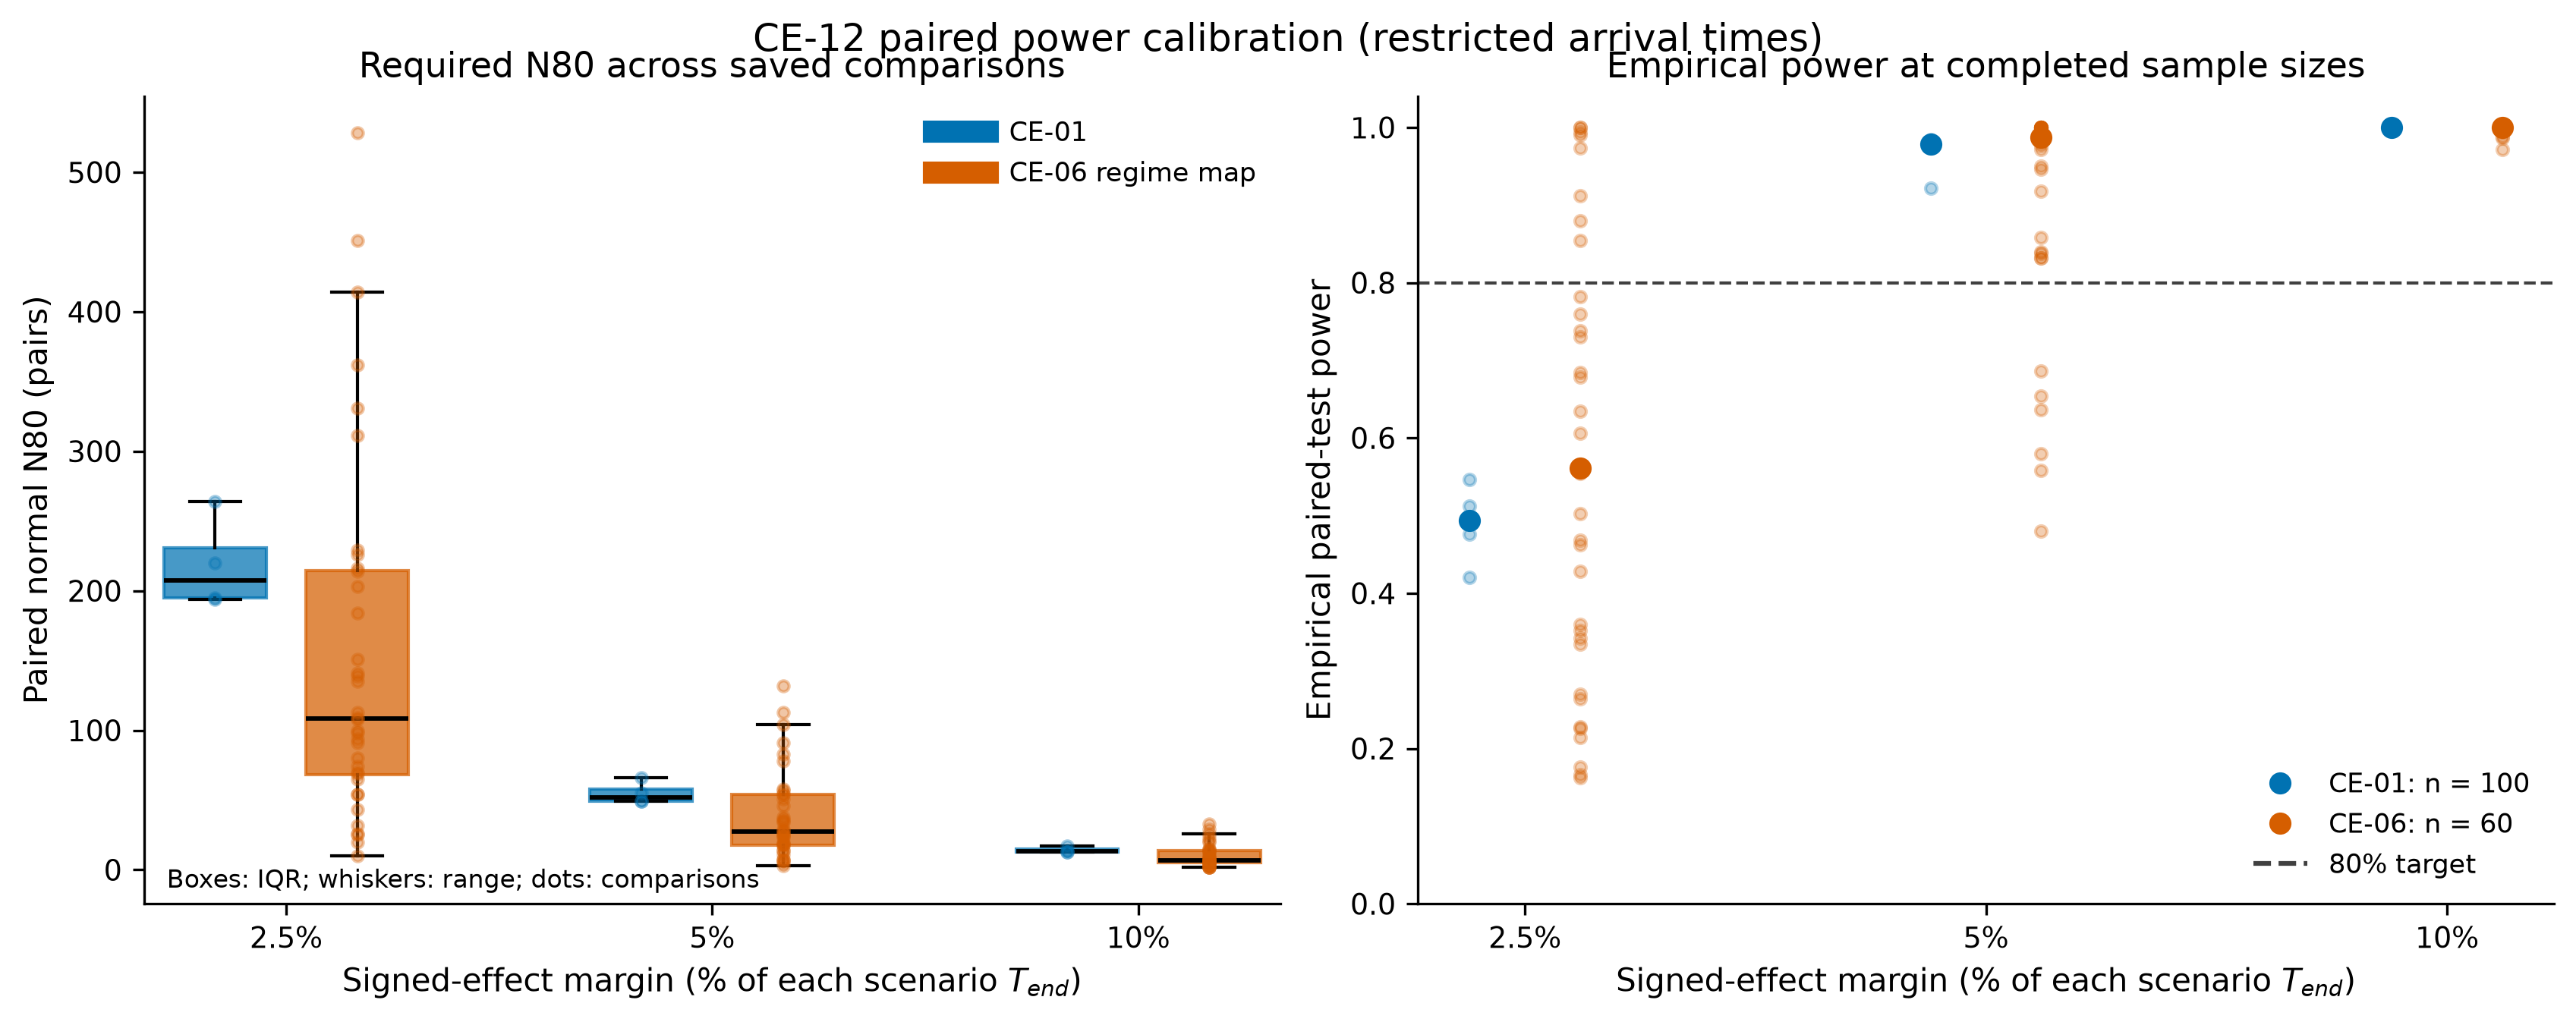
\includegraphics[width=0.94\linewidth]{figures/report_figure.png}
  \caption{Калібрування потрібного розміру вибірки та емпіричної потужності
  за заданими margins; графік має читатися разом із сценарій-залежними
  горизонтами та completion diagnostics у табл.~\ref{tab:completion}.}
  \label{fig:power}
\end{figure}

\section{Аналіз та інтерпретація}\label{sec:interpretation}

Наявні 100 реплікацій CE-01 забезпечують високу чутливість до типового
зміщення 5--10\% горизонту, але для 2.5\% усі plug-in $N_{80}$ перевищують
наявне $n$. У CE-06 навіть висока медіанна потужність не усуває слабких
комірок: для найменшого margin $N_{80}$ сягає 528.

Парування не є автоматично вигідним. Відношення потрібного непарного $N_{80}$
на групу до парного $N_{80}$ було меншим за 1 у 45 зі 120 рядків summary.
Слабка або від'ємна коваріація між $X^*$ та $Y^*$ може збільшувати
$\operatorname{Var}(D)$. Тому розмір вибірки слід планувати за конкретним
режимом, а не за глобальним припущенням про користь парування.

Рис.~\ref{fig:power} та табл.~\ref{tab:completion} разом показують дві різні
вимоги: достатню точність часової метрики й здатність виявити якісну незгоду
щодо досягнення кінцевого шару. CE-12 не встановлює механістичну причину
похибки; він калібрує статистичну спроможність її виміряти.

\section{Значення для двошарової апроксимації та статті}\label{sec:paper}

\begin{itemize}
  \item Твердження про ``малу похибку'' потребує наперед визначеного margin;
  відсутність значущості не доводить еквівалентності.
  \item Дані краще підтримують ефекти 5--10\% горизонту, ніж точність у межах
  2.5\% у кожному режимі.
  \item За цензурування слід спільно подавати $\Delta\mathrm{RMST}$,
  completion, $\Delta$completion і survival/CDF curves.
  \item Додаткові реплікації слід спрямовувати на комірки з найбільшою
  дисперсією або completion discordance, а не розподіляти рівномірно.
\end{itemize}

\section{Обмеження і твердження, яких слід уникати}\label{sec:limits}

\begin{enumerate}
  \item Plug-in аналіз не враховує невизначеність оціненої дисперсії.
  \item Нормальна апроксимація для рекомендованих $N<20$--$30$ ненадійна;
  такі значення є лише грубими орієнтирами.
  \item 500 bootstrap-перевибірок створюють Monte Carlo похибку, особливо
  поблизу порогового рівня потужності.
  \item Корекцію на множинність для 40 порівнянь не застосовано. Окреме
  $p<0.05$ не підтверджує сітково-глобальну гіпотезу.
  \item Не слід називати ці результати потужністю для спостережуваного ефекту:
  signed effect штучно задано рівним margin.
  \item Абсолютні margins і $\Delta\mathrm{RMST}$ не можна безпосередньо
  порівнювати між різними горизонтами.
\end{enumerate}

\section{Практичні рекомендації}\label{sec:recommendations}

\begin{enumerate}
  \item До підтверджувального запуску зафіксувати науково значущі margins.
  \item Збільшити $n$ для CE-01 при 2.5\% та для найслабших комірок CE-06.
  \item Для малого $N$ застосувати simulation-based calibration або
  перевірку стійкості до ненормальності.
  \item Для completion diagnostics визначити первинні контрасти й правило
  множинної корекції до аналізу.
\end{enumerate}

\section{Відтворення}\label{sec:reproduction}

Analysis runner: \path{extrascripts/run_ce12_power_calibration.py}.
Основні результати: \\
\path{output/claude_experiments/ce12_power_calibration/power_summary.csv}, \\
\path{output/claude_experiments/ce12_power_calibration/empirical_power.csv}, \\
\path{output/claude_experiments/ce12_power_calibration/completion_discordance.csv}.
Формули, seed \texttt{812120026}, SHA-256 джерел і статус analysis-only:
\path{output/claude_experiments/ce12_power_calibration/manifest.json}.
Джерела: \path{output/ablation_hazard_placement/final_100/arrival_times.csv}
та \path{output/claude_experiments/ce06_regime_map_full/cells/}.

\end{document}
